%-------------------------------------------------------------------------------
% 请勿删除本注释
% Free Response Question 3
%
% 指引:
% 如在小问之前有通用问题描述,请放置于此
%-------------------------------------------------------------------------------
\begin{figure}[H]
\centering
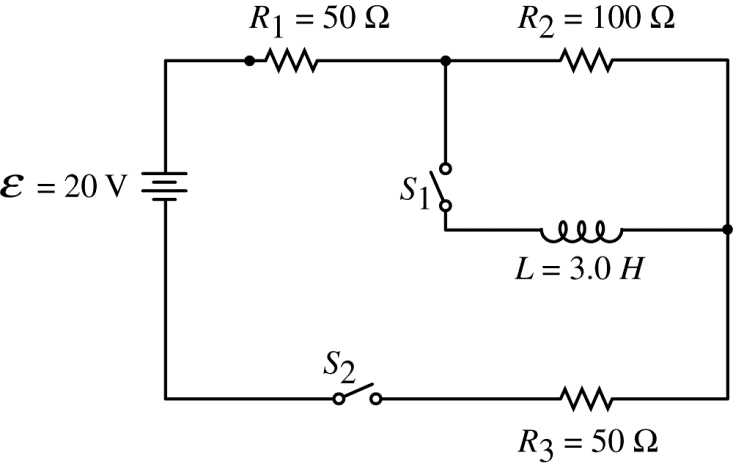
\includegraphics[scale=0.3]{images/img-024-050.png}
\end{figure}

\question
An ideal battery is connected to three resistors, an ideal inductor, and two switches, as shown in the circuit above. Both switches are initially open. Switch $S_{2}$ is then closed.  % 请删除并替换本行,与上一行 \question 之间不要留空行

\begin{parts}

%-------------------------------------------------------------------------------
% 请勿删除本注释
% Part (a)
%
% 指引:
% 如在小问之前有通用问题描述,请放置于此
%-------------------------------------------------------------------------------

\part
Calculate the voltage across resistor $R_{2}$. % 请删除并替换本行,与上一行 \part 之间不要留空行

%-------------------------------------------------------------------------------
% 请勿删除本注释
% Part (b)
%
% 指引:
% 如在小问之前有通用问题描述,请放置于此
%-------------------------------------------------------------------------------

Switch $S_{1}$ is then closed.

\part
Calculate the magnitude of the rate of change of the current through the inductor immediately after switch $S_{1}$ is closed. % 请删除并替换本行,与上一行 \part 之间不要留空行

%-------------------------------------------------------------------------------
% 请勿删除本注释
% Part (c)
%
% 指引:
% 如在小问之前有通用问题描述,请放置于此
%-------------------------------------------------------------------------------

\part
At time $t$ after switch $S_{1}$ is closed, the instantaneous current through resistor $R_{2}$ is measured to be $0.020$ A. % 请删除并替换本行,与上一行 \part 之间不要留空行
\begin{subparts}
\subpart Calculate the current through resistor $R_{3}$ at time $t$.
\subpart Calculate the energy stored in the inductor at time $t$.
\end{subparts}

%-------------------------------------------------------------------------------
% 请勿删除本注释
% Part (d)
%
% 指引:
% 如在小问之前有通用问题描述,请放置于此
%-------------------------------------------------------------------------------
After a long time, the currents reach a steady value. Switch $S_{2}$ is then opened.

\part
Calculate the current through the inductor immediately after switch $S_{2}$ is opened. % 请删除并替换本行,与上一行 \part 之间不要留空行

%-------------------------------------------------------------------------------
% 请勿删除本注释
% Part (e)
%
% 指引:
% 如在小问之前有通用问题描述,请放置于此
%-------------------------------------------------------------------------------

\part
Write, but do NOT solve, a differential equation that can be used to determine the current through resistor $R_{2}$ at time $t$ after switch $S_{2}$ is opened. % 请删除并替换本行,与上一行 \part 之间不要留空行

%-------------------------------------------------------------------------------
% 请勿删除本注释
% Part (f)
%
% 指引:
% 如在小问之前有通用问题描述,请放置于此
%-------------------------------------------------------------------------------

\part
Using the differential equation from part (e), derive an expression for the current through resistor $R_{2}$ as a function of time $t$ after switch $S_{2}$ is opened. % 请删除并替换本行,与上一行 \part 之间不要留空行

\end{parts}
